\begin{frame}
    \frametitle{Introducción}
    \begin{itemize}
        \item ZeroMQ \red{no} es un demonio.
        \item ZeroMQ \red{no} es un servidor.
        \item ZeroMQ es una biblioteca de mensajes.
    \end{itemize}
\end{frame}

\begin{frame}
    \frametitle{Introducción}
    \begin{center}
        Principalmente es un nueva \blue{capa de red} que actúa
        como un sistema de \blue{sockets},
        capaz de hacer concurrencia, encolamiento, etc.
    \end{center}
\end{frame}

\begin{frame}
    \frametitle{Introducción}
    \begin{itemize}
        \item Comunicación entre colas:
        \begin{itemize}
            \item Computadores en una Red.
            \item Procesos en un computador.
            \item Hebras en un proceso.
            \item Combinaciones.
        \end{itemize}
    \end{itemize}
\end{frame}


\begin{frame}
    \frametitle{Introducción}
    \framesubtitle{Modelos}
    \begin{center}
        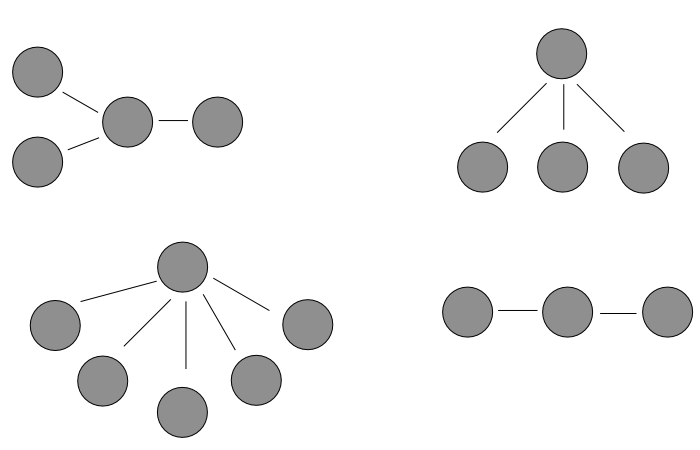
\includegraphics[width=0.6\textwidth]{img/modelos}
    \end{center}
\end{frame}

\begin{frame}
    \frametitle{Introducción}
    \framesubtitle{Performance}
    \begin{itemize}
        \item Sin overhead de protocolo.
        \item Uso eficiente de reliable Multicast.
        \item Uso inteligente de lotes de mensajes con TCP/IP (minimizando overhead y llamadas a sistema).
    \end{itemize}
\end{frame}

\begin{frame}
    \frametitle{Introducción}
    \begin{itemize}
        \item Simple
        \begin{itemize}
            \item API
        \end{itemize}
        \item Escalabilidad
        \begin{itemize}
            \item Poder de un socket.
            \item Balance de carga.
            \item Diseño sin ``broker''.
        \end{itemize}
    \end{itemize}
\end{frame}
